\chapter{Theory}
\section{The Model Organism/Study Animal}
Euryhaline, osmoconformer, closes valves in periods of exposure to brackish/fresh water (low tide), keeping the saline pallial/mantle fluid as the immediate surrounding environment. Becomes isosmotic with the pallial fluid (Gilles, 1972). In long exposures (> 75 hours) or by puncturing/keeping the valves prised they are forced to pump water, and the hemolymph rapidly conforms to the exterior osmolarity. Short said: is an osmoconformer that behaviorally protects itself from short-term exposures to hypo-osmotic conditions rather than physiologically (Davenport, 1979). Relevant for the osmolarity of buffers/solutions used.

\begin{figure}[H]
    \centering
    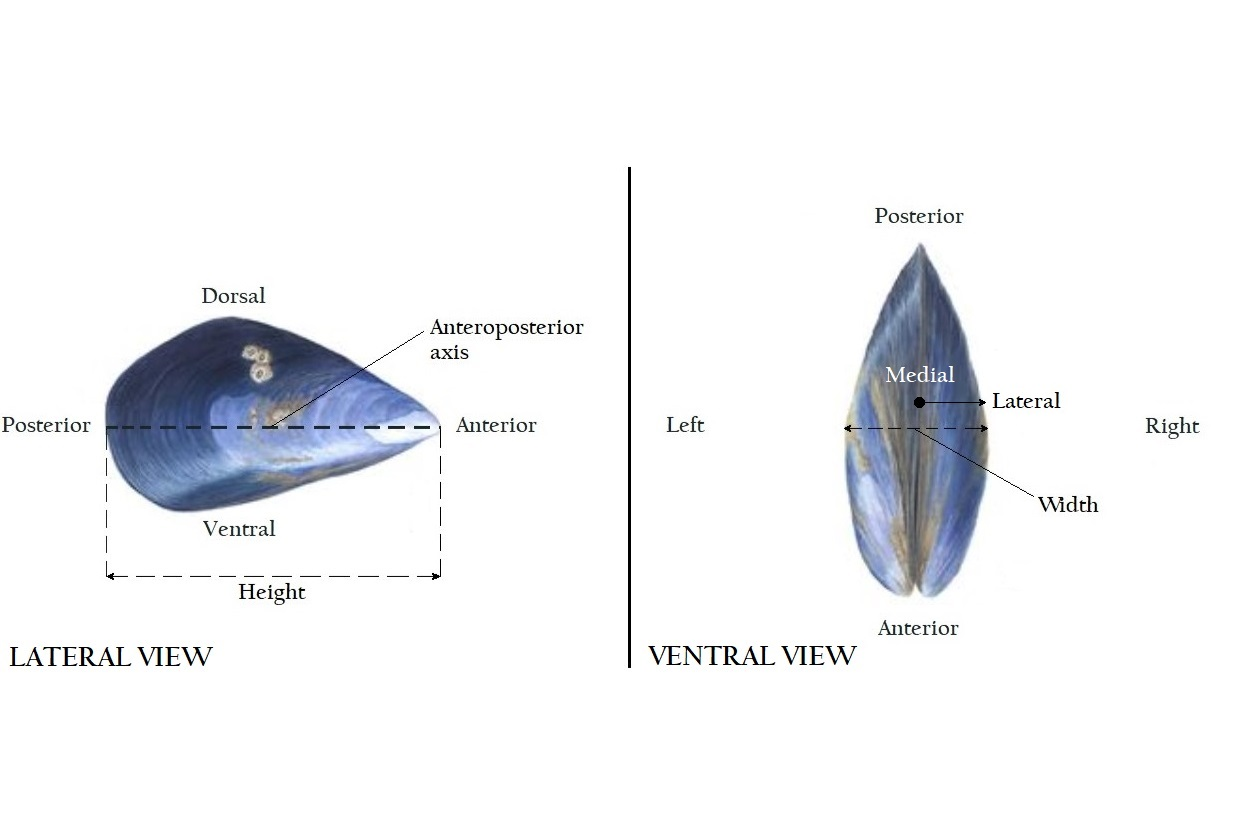
\includegraphics[width=\textwidth]{figures/Anatomy/M_edulis_anatomical_axis_lateral.jpg}
    \caption{The figure caption depends on if it ends up here, or in the material and method. Write when decided. The illustration was adapted from an artistic work by Abby Towne, A. Towne Design with permission.}
    \label{fig:anatomical_axis}
\end{figure}


\subsection{Classification of the haemocyte subpopulations of \emph{M. edulis}}
Since the first written account on the subject (\cite{Cuenot1891}), several authors have devoted their attentions to developing a unifying classification system for the amoebocytic blood cells of bivalve mollusks, more commonly known as haemocytes (\cite{Cheng1980, delaBallina2022}). Belonging to the bivalve familiy \emph{Mytilidae}, the haemocytes of \emph{Mytilus edulis}, \emph{Mytilus galloprovincialis} and several other commercially important species of the genus \emph{Mytilus} have been encompassed by these efforts, creating a substantial pool of literature on the haemocytes of this genus alone. Despite a lack of consensus for any unifying classification system for the haemocytes of this phylum at large, the literature that exists on the haemocytes of \emph{M. edulis} is generally in agreement.

The first effort to classify the haemocytes of \emph{M. edulis} was made by Moore and Lowe (1977). Much like the other attempts to classify bivalve haemocytes at the time, this classification was based on the morphofunctional aspects of these cells - a system that has been extensively reviewed by Hine (1999). Moore and Lowe constructed a simple classification based on static morphological and ultrastructural characteristics of the haemocytes, combined with their phagocytic capacities (\cite{Moore1977}). From routine cytological staining, they identified three haemocyte subpopulations (or cell types): "(1) small basophilic hyaline cells or lymphocytes, (2) larger basophilic hemocytes with varying degrees of irregular cytoplasmic granulation and vacuolation, and (3) eosinophilic granular haemocytes or granulocytes" (\cite{Moore1977}). The small blast-like cells (4-6 \micro m) were generally spherical in outline, had a scant thin rim of basophilic hyaline (read: transparent) cytoplasm and a spherical nucleus. The larger basophilic cells (7-10 \micro m) had lower N:C ratios, but displayed a less intensely stained basophilic cytoplasm with a more irregularly shaped nucleus. The eosinophilic granulocytes were the largest cell type identified (7-12 \micro m). They had a regular spherical appearance, further characterized by a small round nucleus, low N:C ratio, and a cytoplasm filled with spherical eosinophilic granules (0.5-1.0 \micro m). Their electron-microscopical examinations confirmed the existence of three ultrastructurally distinct cell types. Except for a few mitochondria, the blast-like cells contained a scarcity of organelles and granules. This was in sharp contrast to the larger basophilic cells, which contained Golgi apparatus, phagosomes and smaller granular inclusions - possibly representing primary lysosomes. A phagocytosis assay with experimentally injected carbon particles revealed that both granular cell types had phagocytic properties, while the small blast-like cells did not show evidence for this capacity. To reflect this functional evidence, the small blast-like haemocytes were referred to as small lymphocytes, while the larger granular basophilic haemocytes were classified as phagocytic macrophages.

If reduced it's static morphological criteria, Moore and Lowe's classification of \emph{M. edulis} haemocytes coincides with the original system of Cúenot (1891). This system generally recognized three haemocyte types: "(1) finely granular haemocytes, (2) coarsely granular haemocytes and (3) cells with very little cytoplasm surrounding the nucleus" (\cite{Cheng1984}). Leaning towards a two-categorical classification (hyalinocytes and granulocytes), Cheng (1981) argued that a distinction between the basophillic and eosinophilic granulocytes of \emph{M. edulis} was artificial, as the reviewer saw them as being the immature and mature stages of the same cell type (granulocyte), respectively. From observations of what resembled intermediate stages between the blast-like and larger basophilic cells, Moore and Lowe (1977) argued that the basophilic cells constituted an ontogenic developmental series, with the larger phagocytic macrophages representing the final stage of differentiation. This was further supported by observations of blast-like cells with mitotic figures, suggesting that it could be the stem cell of this developmental series (\cite{Moore1977}). Since a few smaller eosinophilic granulocytes (5-7 \micro m) were observed, they were believed to represent a distinct growth series. As noted by Cheng (1981), this account is not based on direct evidence, but is rather interpretive evaluations of their findings. Haemocyte classification should be based on their ontogenic lineages, but 


Moore and Lowe (1977) had argued tha



These were postulated to make up two distinct growth series


, but is rather interpretive evaluations from observations of small or intermediate phenotypes with mitotic figures (or a lack thereof) and changes accompanied by increasing cell sizes in both basophilic and eosinophilic haemocytes.



Functional classification based on phagocytic capacity: Differences in phagocytosis between granulocytes and agranular haemocytes may be related to the type of phagocytosed particles involved, rather than differences in phagocytic ability.

Hine (1999) about "blast-like cells": Basophilic cytoplasm, suggesting presence of free ribosomes and immaturity. Their lack of cytoplasmic organelles preclude a secretory of phagocytic function.

Ontogeny by the use of monoclonal antibodies \cite{Noel1994} and \cite{Dyrynda1997}.

Conclude with something like this:
Except for a difference in terminology/naming, based on the ultra-structure and cytologic staining of these haemocytes, they are referring to the same cells. 


\begin{table}[ht!]
	\centering
	\caption{Classification of hemocyte subpopulations in \emph{Mytilus edluis}.}
	\label{tb:hemocyte_classification}
 \resizebox{\linewidth}{!}{
	\begin{tabular}{lcccccl}
		\toprule
		\multirow{2}{*}{Number of} & \multirow{2}{*}{Eosinophils} & \multicolumn{2}{c}{Basophils} & \multicolumn{2}{c}{Hyalinocytes} & \multirow{2}{*}{Reference} \\
  \cmidrule(lr){3-4} \cmidrule(lr){5-6}
        supopulations (n) & & B1 & B2 & H1 & H2 & \\
        \midrule
		3 & Granulocytes & Large phagocytic macrophages & Small lymphocytes & & & \cite{Moore1977} \\
        3 & Granulocytes & Granulocytes (small granules) & Small agranular & & & \cite{Pipe1997} \\
        3 & Granulocytes & Granulocytes & Agranulocytes & & & \cite{Renwartz1990} \\
        
        
  
		\bottomrule
  \multicolumn{6}{c}{\footnotesize G, granulocyte; H, hyalinocyte; sH, small hyalinocyte; B, blast-like cells; AG, agranulocyte; haemoblast-like cells, prohaemocytes, SemiG, semigranulocyte; }
	\end{tabular}
 }
\end{table}

Blast-like cells are better, which are also referred to as, basophils, haemoblast-like, small hyalinocytes in various bivalve species.

Moore and Lowe (1977) Electron micrograph study
(1) small basophilic hyaline cells or lymphocytes
(2) larger basophilic hemocytes with varying degrees of irregular cytoplasmic granulation and vacuolation. More irregular shaped nucleus. Granules irregular in shape.
(3) eosinophilic granular hemocytes or granulocytes

Moreover, the small hyaline cells did not in general display any evidence of phagocytic activity, although some of the hemocytes of intermediate size did contain ingested carbon particles. On this basis, the basophilic cells have been subdivided into small non-phagocytic lymphocytes and larger phagocytic macrophages. 

Renwartz (1990) Internal defence system of Mytilus edulis \cite{Renwartz1990}
Confirmed the occurrence of two types of basophillic hemocytes: both small agranular cells and granular basophils, or so-called macrophages.

Pipe (1997) Percoll, electron microscopy and light microscopy (Wright's)
(1) mainly small agranular cells 
(2) granular cells with small granules (0.2-0.3 um)
(3) granulocytes with larger granules (0.5-1.5 um)

When taken together with light microscopy examinations, cell types 1 and 2 are both basopilic, and those with larger granules that separated out in the highest density layer are eosinopillic granulocytes.

Pipe (1990), Electron microscopy w/ lectin binding
Haemocytes fixed in suspension showed 3 basic types of ultrastructural morphology and were classified as:
(1) hyalinocytes
(2) granulocytes with small (0.2-0.3 um) granules
(3) granulocytes with large (0.5-1.5 um) granules

Rasmussen (1985), Electron and light microscopy (May Grünwald) \cite{Rasmussen1985}
The granulocytes had either acidophilic granules, basophilic granules, or a mixture of both. Could be divided into two populations:
Electron micrographs revealed granular and agranular hemocytes:
(1) Small granulocytes (6.9-8 um): lobulate nucleus, varying numbers of rather small round specific granules in the paranuclear cytoplasm. Had sometimes cytoplasmic protrusions (pseudopodia)
Large granulocyte (8-11 um): nucleus not lobulate, cytoplasm completely filled with specific granules, larger than those of the small granulocytes.
(3) Agranular hemocytes were very small (5.0-5.9 um) with an intense basophilic cytoplasm almost masking the nucleus (bean-shaped or lobulate).

Did not perform light microscopy examinations to correlate ultrastructure to Wright's-Giemsa staining profiles.



FLOW CYTOMETRY and LIGHT MICROSCOPY

Le Foll (2010), FCM and microscopy \cite{LeFoll2010}
(1) Basophils, some with a few large granules upon osmotic swelling
(2) Hyalinocytes, often spread cells, low N:C ratio, often clear vacuoles/phagosomes. (These are spread basophils). Cytoplasm barely visible.
(3) Eosinophilic granulocytes

Parisi (2008) Flow cytometry and light microscopy (Mytilus galloprovencialis)
Their FSC vs. SSC density plots revealed three distinct subpopulations (which was confirmed by light microscopy):
(1) agranular cells
(2) small granulocytes
(3) large granulocytes



ONLY LIGHT MICROSCOPY

Friebel and Renwratz (1995), Percoll separation and light microscopy. 
When the hemocytes of Mytilus edulis were stained with MG dye, all cells contained either basophilic or eosinophilic cytoplasm (Friebel and Renwartz, 1995). (Y) :) They did however note that there were smaller and larger basophilic haemocytes

Wootton (2003), light microscopy
Distinguished three cell types in the haemolymph of \emph{M. edulis}:
(1) Agranular basophils or hyaline cells: ca. 3–4 um, high nucleus:cytoplasm ratio and lack/low abundance of cytoplasmic granules and organelles
(2) Granular basophils: were slightly smaller than the eosinophilic haemocytes (ca. 7–8 um diameter), but were similar in terms of their N:C ratio
(3) the largest haemocytes (ca. 10–12 um diameter), characterized by large numbers of eosinophilic granules and a round nucleus. Generally low N:C ratio

\section{The role of hemocytes}
Hemocytes also (in addition to lung and digestive gland) showed high expression levels (of initiator and executioner caspases), probably due to the role of apoptosis in the defense against pathogens. Because bivalves are highly susceptible to climate changes, pollutants and pathogens, it  could be suggested that a strong apoptotic process may be necessary to ensure body homeostasis. (Romero, 2011). See page 11 of (New Insights into the Apoptotic Process in Mollusks: Characterization of Caspase Genes in Mytilus galloprovincialis) for greater detail and references.

Relocate the article about the role of hemocytes in wound-healing in mussels.

The total hemocyte count (THC) decreased by 66\% after a bacterial injection \cite{Parisi2008}. This could actually be to hemocyte aggregation in response to the needle injection itself.

I

\section{Bivalve hemocytes as \emph{in vivo} and \emph{in vitro} model systems}
Used as membrane integrity model system.

Introduce ToPro-3, Calcein AM (Calcein acetoxymethyl) and Apo-15 (\cite{Barth2020}) and their principle of staining, i.e., dye exclusion, cell-permeable (non-specific esterase substrate) and binding to phosphatidyl serine externalized during programmed cell death.

Theory behind Annexin-V/Apo-15: Annexin V
has affinity for phosphatidylserine, which is externalized to the
outer layer of the plasma membrane in the earlier stages of apoptosis. Annexin V also binds internal phosphatidylserine in permeable membranes, i.e. dead cells. Thus, dead cells are Apo-15+ ToPro3+, while the early apoptotiv cells are only Apo15+.